% this file is called up by thesis.tex
% content in this file will be fed into the main document

%: ----------------------- name of chapter  -------------------------
\chapter{Teori} % top level followed by section, subsection
\label{teori}

%: ----------------------- paths to graphics ------------------------
\ifpdf
    \graphicspath{{3_theory/figures/PNG/}{3/figures/PDF/}{3/figures/}}
\else
    \graphicspath{{3_theory/figures/EPS/}{3/figures/}}
\fi

\graphicspath{{3_theory/figures/}{3/figures/}}

%: ----------------------- contents from here ------------------------

\section{Problemet med skadegörelse}

Sannolikheten för vandalisering av busshållplatser ökar när det är mörkt ute och under nattetid just på grund av att akten inte skall upptäckas. Det visar sig att brottsligheten minskar och bättre uppförande finns hos människor i ett område enbart om där finns en skylt som säger att området är övervakat. Gruppen bygger upp denna uppfattning eftersom Brottsförebyggande rådet BRÅ skriver på sin hemsida \cite{bra} att kameraövervakning i brottsförebyggande syfte blir allt mer vanligt i Sverige. Speciellt när kameraövervakningslagen trädde i kraft i juli 2013, har det underlättat för installationer av kameraövervakningar. Gruppen refererar även till egna erfarenheter om områden och tider på dygnet då människor känner sig otrygga vid busshållplatser. 

\begin{figure}[h]
  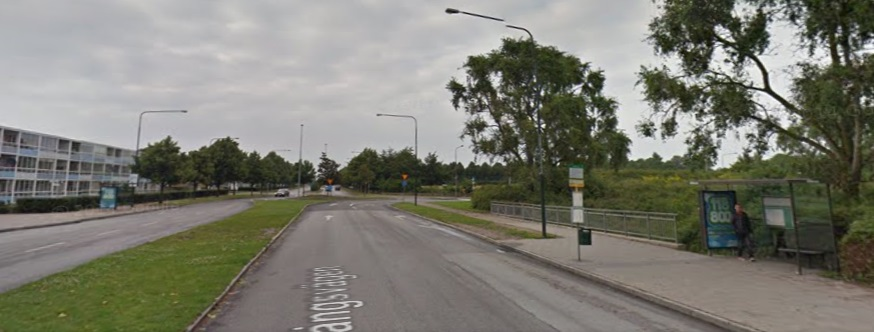
\includegraphics[width=\linewidth]{lind.jpg}
  \caption{En obevakad hållplats i Malmös stadsdel Lindängen. (Google Maps: Lindängen - Malmö)}
  \label{fig:lind}
\end{figure}

Busshållplatser som är oövervakade där människor kommer och går i intervaller, kan utsättas för skadegörelse där exempelvis glaset krossas eller otillåten vandalisering görs. Denna skadegörelse kostar samhället pengar och fortsätter än idag att kosta samhället pengar då där inte finns någon bra lösning på problemet än. Tryggheten skulle möjligtvis öka då busshållplatsen är övervakad.\\


En busshållplats som är övervakad dygnet kommer att registrera mycket data och är således ineffektiv lösning. Kameran som kommer användas i syftet att övervaka busshållplatsen ska enbart aktivt övervaka busshållplatsen då specifika villkor är uppfyllda. Villkoren är då en människa är närvarande, rörelse registreras eller vandalisering mot busshållplatsen utförs. Om inget villkor är uppfyllt så kommer systemet att vara i ett passivt tillstånd och enbart lyssna på förändringar.\\

Sensorer används för att lyssna till förändrings hos omgivningen. Dessa förändringar kommer att utvärderas något och jämföras med fördefinierade villkor för systemet. När ett villkor är uppfyllt så kommer systemet att aktiveras och börja registrera data och skicka denna data via internet till en server för datalagring.\\

% ---------------------------------------------------------------------------
%: ----------------------- end of thesis sub-document ------------------------
% ---------------------------------------------------------------------------

